\documentclass{article}

\usepackage{graphicx}
\usepackage{tikz}
\usepackage{tikzsymbols}
\usetikzlibrary{calc,patterns,shapes.geometric}
\pagestyle{empty}
\usepackage[margin=0pt]{geometry}
\geometry{papersize={14in,12in}}

\def\centerarc[#1](#2)(#3:#4:#5){\draw[#1] ($(#2)+({#5*cos(#3)},{#5*sin(#3)})$) arc (#3:#4:#5);}

\begin{document}
	\begin{figure}
		\centering
		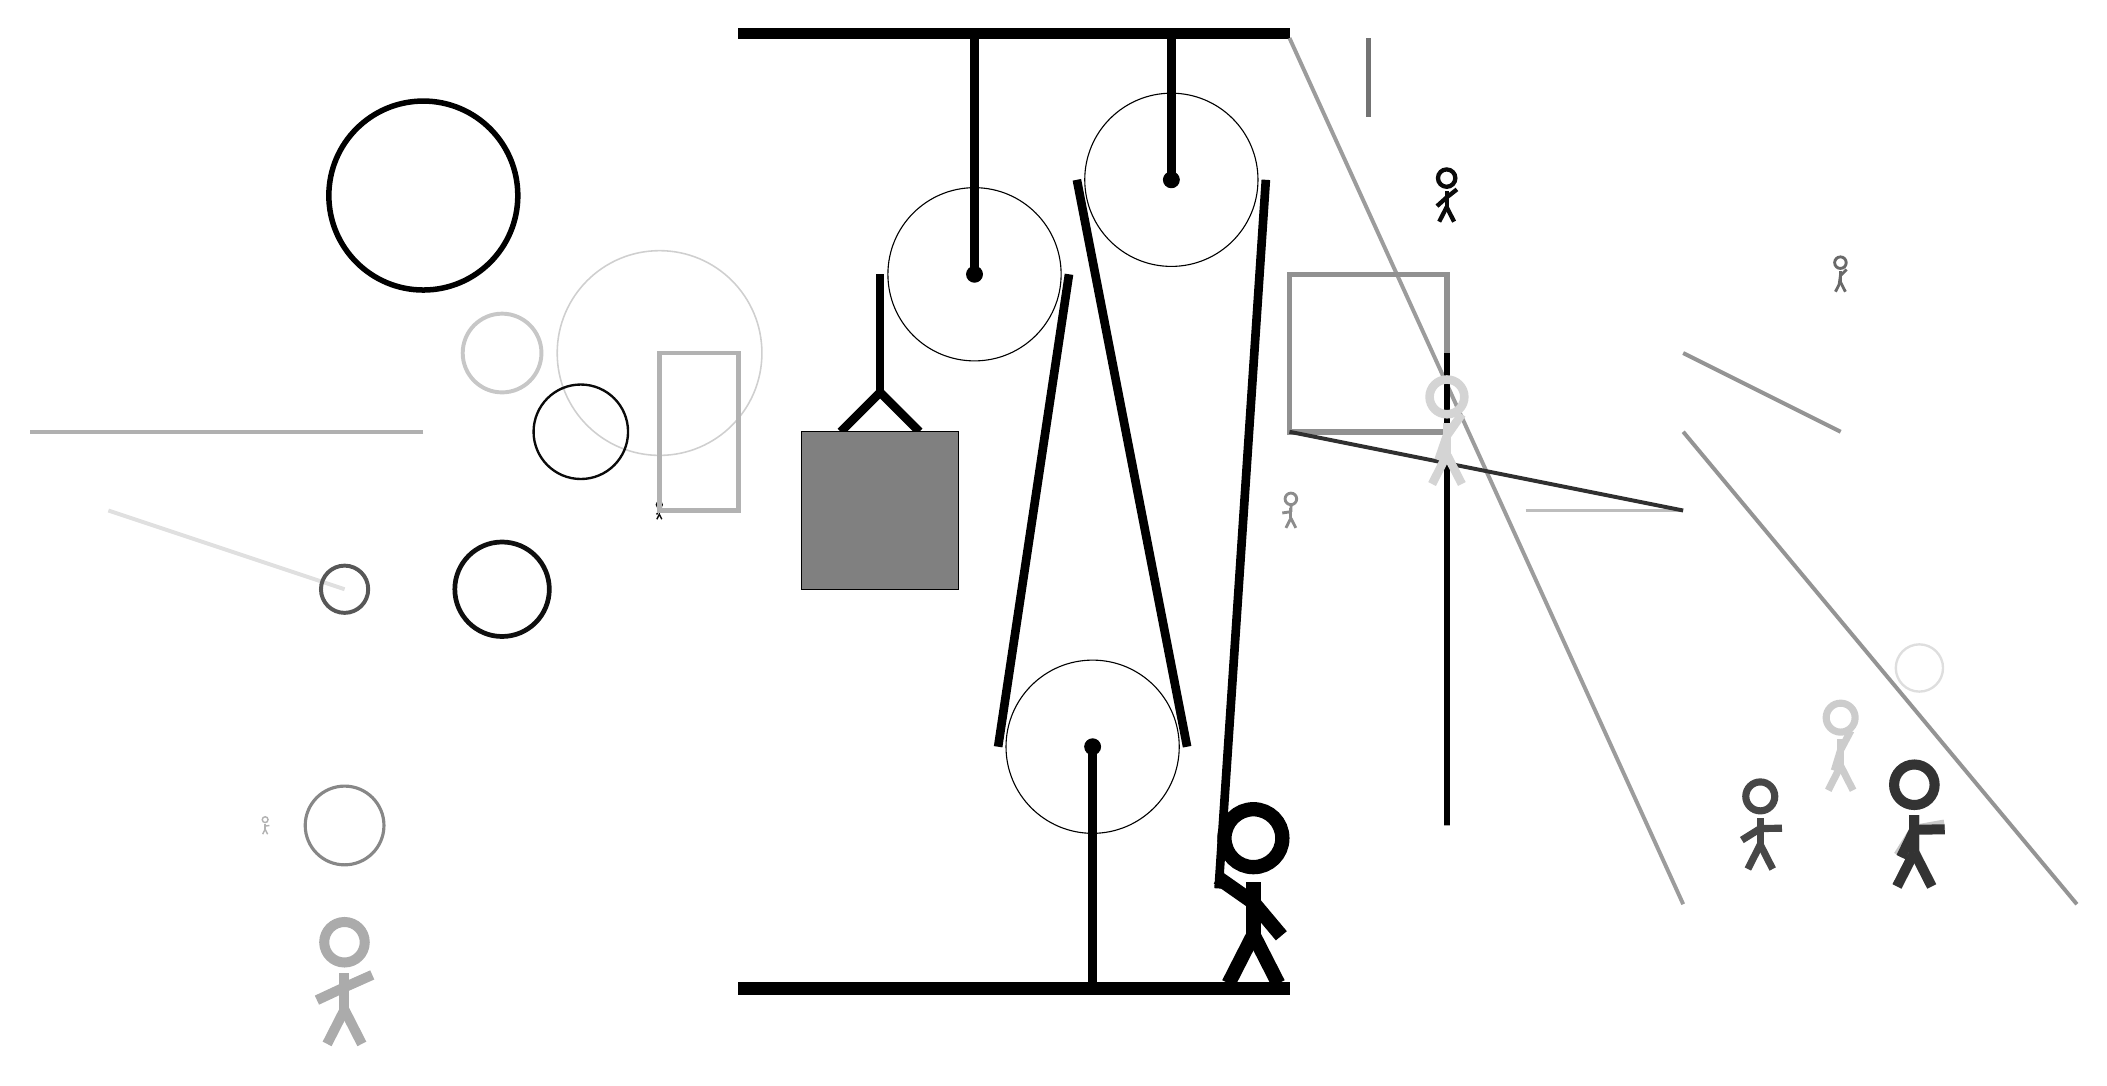
\begin{tikzpicture}
			%%%%% START %%%%%
			
			\draw[fill=black] (-2, 9) rectangle (5, 9.125);
			
			\draw (1, 6) circle (1.1);
			\draw[fill=black] (1, 6) circle (0.1);
			\draw[line width=1.1mm]  (1, 9) -- (1, 6);
			
			\draw[fill=white](2.5, 0) circle (1.1);
			\draw[fill=black] (2.5, 0) circle (0.1);
			\draw[line width=1.1mm]  (2.5, -3) -- (2.5, 0);
			
			\draw[fill=white](3.5, 7.2) circle (1.1);
			\draw[fill=black] (3.5, 7.2) circle (0.1);
			\draw[line width=1.1mm] (3.5, 9) -- (3.5, 7.2);
			
			\draw[line width=1.1mm] (-0.7, 4.0) -- (-0.2, 4.5) -- (0.3, 4.0);
			\draw[fill=black!50] (-1.2, 4.0) rectangle (0.8, 2.0);
			
			\draw[line width=1.1mm] (-0.2, 6) -- (-0.2, 4.5);
			\centerarc[line width=1.1mm](1, 6)(0:180:1.2000000000000002);
			\draw[line width=1.1mm](2.2, 6) -- (1.3, 0);
			\centerarc[line width=1.1mm](2.5, 0)(180:360:1.2000000000000002);
			\draw[line width=1.1mm](3.7, 0) -- (2.3, 7.2);
			\centerarc[line width=1.1mm](3.5, 7.2)(0:180:1.2000000000000002);
			\draw[line width=1.1mm](4.7, 7.2) -- (4.1, -1.8);
			
			\node at (4.5, -1.9) {\Strichmaxerl[10][-35][-50]};
			
			\node[line width=0.4mm, color=black!96] at (-3, 3) {\Strichmaxerl[1][49][39]};
			
			\draw [line width=0.2mm, color=black!19](-3, 5) circle (1.3);
			\draw[line width=0.5mm, color=black!42](10, 4) -- (15, -2);
			\node[line width=0.5mm, color=black!96] at (7, 7) {\Strichmaxerl[3][42][38]};
			\draw[line width=0.5mm, color=black!39](10, -2) -- (5, 9);
			
			\draw[line width=0.7mm, color=black!43] (7, 6) rectangle (5, 4);
			
			\draw[line width=0.5mm, color=black!26](8, 3) -- (10, 3);
			
			\draw [line width=0.4mm, color=black!47](-7, -1) circle (0.5);
			\draw[line width=0.6mm, color=black!55] (6, 9) rectangle (6, 8);
			
			\draw [line width=0.3mm, color=black!13](13, 1) circle (0.3);
			\node[line width=0.7mm, color=black!72] at (11, -1) {\Strichmaxerl[5][32][1]};
			
			\draw[line width=0.5mm, color=black!12](-7, 2) -- (-10, 3);
			\draw[line width=0.5mm, color=black!31](-6, 4) -- (-11, 4);
			
			\draw[line width=0.5mm, color=black!81](5, 4) -- (10, 3);
			\draw [line width=0.5mm, color=black!66](-7, 2) circle (0.3);
			\draw [line width=0.7mm, color=black!100](-6, 7) circle (1.2);
			
			\node[line width=0.2mm, color=black!21] at (13, -1) {\Strichmaxerl[7][58][10]};
			
			\draw[line width=0.5mm, color=black!42](10, 5) -- (12, 4);
			\node[line width=0.6mm, color=black!80] at (13, -1) {\Strichmaxerl[7][64][1]};
			\draw[line width=0.7mm, color=black!100] (7, -1) rectangle (7, 5);
			\draw[line width=0.6mm, color=black!30] (-3, 5) rectangle (-2, 3);
			\node[line width=0.3mm, color=black!59] at (12, 6) {\Strichmaxerl[2][82][44]};
			\draw [line width=0.6mm, color=black!94](-5, 2) circle (0.6);
			\node[line width=0.4mm, color=black!17] at (7, 4) {\Strichmaxerl[6][71][55]};
			\node[line width=0.3mm, color=black!33] at (-7, -3) {\Strichmaxerl[7][25][24]};
			
			\node[line width=0.7mm, color=black!30] at (-8, -1) {\Strichmaxerl[1][83][8]};
			\draw [line width=0.3mm, color=black!96](-4, 4) circle (0.6);
			\draw [line width=0.5mm, color=black!22](-5, 5) circle (0.5);
			\node[line width=0.5mm, color=black!45] at (5, 3) {\Strichmaxerl[2][8][88]};
			
			\node[line width=0.3mm, color=black!20] at (12, 0) {\Strichmaxerl[5][73][62]};
			
			\draw[fill=black] (-2, -3) rectangle (5, -3.15);
			
			%%%%% END %%%%%
		\end{tikzpicture}
	\end{figure}	
\end{document}